%%%%%%%%%%%%%%%%%%%%%%%%%%%%%%%%%%%%
% Configuración general de página
%%%%%%%%%%%%%%%%%%%%%%%%%%%%%%%%%%%%
\documentclass[10pt,a4paper]{article}
\textheight = 21cm
\textwidth = 15cm
\topmargin = -0.5 cm
\oddsidemargin = 1cm

%%%%%%%%%%%%%%%%%%%%%%%%%%%%%%%%%%%%
% Paquetes
%%%%%%%%%%%%%%%%%%%%%%%%%%%%%%%%%%%%
\usepackage{amsmath}
\usepackage[utf8]{inputenx} % Permite introducir caracteres no ASCII
\usepackage[spanish]{babel} % Hace que los títulos aparezcan en español
\usepackage[pdftex]{graphicx} % uso de graficos en general
\usepackage{subcaption} % poder poner dos graficos como parte de uno
\usepackage{fancyhdr} % encabezado diferente para pag pares e impares
\usepackage{enumerate} % Permite crear listas
\usepackage{adjustbox}
\usepackage{tabu}
\usepackage{multicol} % Permite combinar columnas
\usepackage{multirow} % Permite combinar filas
\usepackage{colortbl} % Colorear celdas
\usepackage{booktabs} % Bordes en tablas
\usepackage{float} % Tablas y figuras flotantes
\usepackage[tablename=Tabla]{caption} % Permite insertar pies de figuras y títulos de tabla
\usepackage{booktabs}
\usepackage{etoolbox} % Permite arreglar errores de ciertos comandos
\usepackage[svgnames, table]{xcolor} % Colores a usar
\usepackage{footnote} % Notas al pie
\makesavenoteenv{tabular} % Permite insertar notas al pie en tablas
\usepackage[colorlinks=true, linkcolor=black, citecolor=black, urlcolor=cyan]{hyperref} % Permite insertar hyperlinks
\usepackage{url} % Corrige errores causados por la presencia de \, _ y otros caracteres en URLs

%%%%%%%%%%%%%%%%%%%%%%%%%%%%%%%%%%%%
% Configuración del formato del doc.
%%%%%%%%%%%%%%%%%%%%%%%%%%%%%%%%%%%%
\patchcmd{\thebibliography}{\section*{\refname}}{}{}{} % Inserta las referencias sin título
\apptocmd{\sloppy}{\hbadness 10000\relax}{}{} % Evita un warning molesto en la bibliografía
\captionsetup{hypcap=false} % Corrige un warning molesto al utilizar hyperref
\AtBeginDocument{
  \let\oldref\ref
  \def\ref{\oldref*}} % Evita la creación de links en donde se llame al comando \ref
\graphicspath{{figuras/}} % Ubicación de los gráficos
\newcommand{\HRule}{\rule{\linewidth}{0.5mm}}
\DeclareGraphicsExtensions{.png,.jpg,.jpeg} % extensiones de las imágenes
\setlength{\parindent}{0.25in}

%%%%%%%%%%%%%%%%%%%%%%%%%%%%%%%%%%%%
% Incluimos el contenido
%%%%%%%%%%%%%%%%%%%%%%%%%%%%%%%%%%%%
\begin{document}

% Title
\begin{center}


\includegraphics[scale=0.1]{itba_logo}
\vspace{1cm}

\textsc{\LARGE Instrumentación Biomédica II - 16.18}\\[0.2cm]
\textsc{\Large Instituto Tecnológico de Buenos Aires}\\[0.2cm]
\vspace{1cm}

\HRule \\[0.2cm]
{ \huge \bfseries Entrega Final - TP Cuatrimestral \\[0.2cm] }
{ \huge \bfseries Grupo n° 6 \\[0.2cm] }
{ \huge \bfseries \textit{Computarized Auditory Brainstem Response Audiometry} (CABRA) \\[0.2cm] }
\HRule \\[1cm]

\vspace{1cm}

\begin{tabular}{| l | c |}
    \hline
    Presentación & \makebox[2cm]{} \\ \hline
    Desarrollo & \makebox[2cm]{} \\ \hline
    Conclusiones & \makebox[2cm]{} \\ \hline
    Nota Final & \makebox[2cm]{} \\ \hline \hline
    Firma y Fecha & \makebox[2cm]{} \\
    \hline
\end{tabular}

\vspace{1cm}
\begin{multicols}{2}

% Author and supervisor
%\large
\begin{tabular}{l l}
  \emph{PRM}  &  Gustavo Panza \\
  \emph{ATP}  &  Ramón Igarreta \\
  \emph{ATP}  &  Franco Perez Rivera \\
  \emph{Ayudante}  &  Bianca Soto Acosta \\

\end{tabular}


% Integrantes
\columnbreak

%\normalsize
\begin{tabular}{l l}
  \emph{Alumnos:}   &  Lucas Franzi \\ &  Gonzalo Grau \\
                    &  Josué Laszeski \\
\end{tabular}

\end{multicols}
\vspace{1cm}

\textbf{Fecha de entrega}: 17/12/2024

\end{center}


%%%%%%%%%%%%%%%%%%%%%%%%%%%%%%%%%%%%%%%%
%                ENCABEZADO
%%%%%%%%%%%%%%%%%%%%%%%%%%%%%%%%%%%%%%%%
\thispagestyle{empty}
\pagestyle{fancy}
\headheight=60pt 	%para cambiar el tamaño del encabezado
\fancyhead[L]{I.B. II - 16.18 - 2024 2C}
% \fancyhead[C]{
\includegraphics[width=20mm]{itba_logo}}
\fancyhead[C]{\textbf{ITBA}}
\fancyhead[R]{Informe CABRA}

\newpage
\tableofcontents
\newpage
\section{Abstract} \label{abstract}

Este trabajo describe el diseño e implementación de un sistema automatizado de audiometría computarizada basado en
la detección y análisis de potenciales evocados auditivos.

El estudio de audiometría busca detectar los umbrales de amplitud sonora a partir de los cuales un sonido es
perceptible para un paciente ante diferentes frecuencias de sonido.
Para ello, se generan estímulos auditivos correspondientes a frecuencias específicas, a diferentes amplitudes, hasta
encontrar el punto umbral.
Técnicas más avanzadas implican el análisis de potenciales evocados auditivos para automatizar la detección de
dichos límites.
Se investigó acerca de los productos más utilizados para realizar este tipo de estudios, y se encontró que los
dispositivos comerciales disponibles son de un elevado costo, además de que no existen alternativas de producción
nacional.

Nuestro proyecto, CABRA (Computer Automated Brainstem Response Audiometry), tiene como objetivo realizar audiometrías
basadas en análisis de potenciales evocados auditivos del tronco encefálico a un bajo costo.
Para ello, se diseñó un sistema de hardware basado en un microcontrolador ESP32-S2, el cual recibe una señal
proveniente del tronco encefálico del paciente (mediante electrodos colocados superficialmente), previamente
filtrada y amplificada, y la digitaliza para su posterior procesamiento.
Luego, las señales recibidas son procesadas digitalmente por un software de escritorio, el cual se encarga de
realizar el estudio completo de audiometría (generando los estímulos auditivos correspondientes) analizando las
señales fisiológicas obtenidas.

Este sistema es modular, amigable al usuario, rápido, y ampliamente configurable.
Además de proveer una herramienta para evaluar la integridad de las vías auditivas del paciente, CABRA permite
acelerar el estudio de audiometría al guiar al usuario en la búsqueda de los umbrales de percepción mediante un
sistema experto.

A futuro, como posibles mejoras, podría modificarse el sistema de adquisición de señales, junto con el de generación
de estímulos, para disminuir la latencia en el muestreo.
Con respecto al software, el sistema experto podría optimizarse mediante algoritmos de machine learning.
Además, la presentación de la carcasa podría ser más compacta y ergonómica.


\section{Introducción} \label{introduccion}

La audiometría es un estudio médico funcional tiene como objetivo evaluar la percepción sonora de un paciente.
Es de particular interés clínico, ya que permite detectar y caracterizar distintos tipos de hipoacusias.

Específicamente, se busca detectar a partir de qué intensidad de sonido (comunmente llamada SPL, por las siglas en inglés de \textit{sound pressure level}) en decibeles [dB] comienza a ser detectable un sonido de una frecuencia específica en Hertz [Hz].
Para ello, se estimula al paciente con señales auditivas en un barrido de frecuencias y SPL, pidiendo que se indique la intensidad para el que cada frecuencia deja de ser perceptible.
De esta manera, se genera un gráfico denominado audiograma, que indica los límites perceptibles en dB vs. Hz.

El estímulo auditivo utilizado suele ser una secuencia de clics cortos, cuya forma de onda es senoidal pura y de frecuencia controlada.
Este sonido se hace llegar al paciente por vía aérea y vía ósea, para poder así discernir entre hipoacusias conductivas (generadas por patologías en el oído medio) y neurológicas (por deficiencias en el oído interno o el sistema nervioso central).
Se utilizan audífonos para la conducción aérea, y dispositivos vibrantes presionados contra las sienes para la ósea.

Si bien la audiometría tradicional requiere de la participación activa del paciente, requiriendo que se indique expresamente la percepción de cada estímulo, existen técnicas que permiten inferir esta condición en forma objetiva e independiente del sujeto.
Una de las más utilizadas consiste en el procesamiento de señales de respuesta auditiva del tronco encefálico (ABR, por sus siglas en inglés para \textit{auditory brainstem response}).
Esta se obtiene midiendo la diferencia de potencial entre dos electrodos contralaterales, colocados en las apófisis mastoideas, y tomando como referencia el tercer ojo.
Debido a que esta es una señal particularmente ruidosa, se la procesa promediando los resultados de múltiples mediciones para iguales condiciones experimentales.
Como resultado, se obtiene una forma de onda tipificada, con picos y valles conocidos \cite{shojaeemend_automated_2018}.
Mediante técnicas de procesamiento digital, se puede estimar la percepción sonora para cada frecuencia en función del SPL, independizándose de participación del paciente. \cite{silva_objective_2009}.

Según un reciente artículo de \textit{Market Research and News} \cite{news_abr_nodate}, el mercado de dispositivos de audiometría basada en ABR se encuentra a la alza.
Estos equipos son de particular interés para los casos en los que el paciente no puede acceder a una audiometría convencial que requiera de su participación, como es el caso de los infantes.
Es especialmente relevante detectar hipoacuasias en infantes de manera temprana, debido a que de ser necesario el uso de implantes cocleares, estos se adoptan en forma óptima durante los primeros 12 a 36 meses.
Por este motivo, muchos países están adoptando programas de evaluación auditiva generalizada, contribuyendo así al interés del mercado en productos aptos para infantes.

A día de hoy, los principales desarrolladores de este tipo de dispositivos son Welch Allyn y Natus, ambas basadas en los EE. UU. Sin embargo, se prevé un crecimiento de la industria para los próximos 10 años en el mercado sudamericano, particularmente en México, Brasil, y Argentina \cite{news_abr_nodate}.
Para este mercado, es vital considerar la accesibilidad en costo, para permitir así su uso en zonas carenciadas.
Mientras que en norteamérica esto no es una prioridad, en Argentina es uno de los puntos clave.

En este contexto, surge CABRA (Computer Automated Brainstem Response Audiometry), un sistema de audiometría basado en ABR que busca ser accesible en costo y fácil de usar.
Mediante este dispositivo, se pueden realizar un estudio completo de audiometría registrando las respuestas del tronco encefálico a estímulos auditivos, sugerir los umbrales de percepción, y generar un audiograma.
Además, se busca que el sistema sea modular, permitiendo la incorporación de mejoras y adaptaciones en el futuro.

\subsection{Objetivos del proyecto} \label{objetivos}
\begin{itemize}
    \item Una interfaz gráfica para el control de los estímulos y la visualización de los resultados
    \item Generación de estímulos por vía aérea y ósea
    \item Correcta adquisición de la señal de ABR mediante un preprocesamiento analógico y un posterior filtrado digital
    \item Procesamiento de la señal de ABR para la detección de los umbrales de percepción
    \item Automatización de la generación de estímulos necesarios para completar una audiometría
    \item Minimización del tiempo de estudio mediante selección inteligente de estímulos
    \item Integración del hardware en una carcasa ergonómica y compacta
\end{itemize}

\section{Marco teórico} \label{marco_teorico}

\subsection{Potencial evocado auditivo}

El potencial evocado auditivo es una señal eléctrica generada por el nervio auditivo y distintas partes del encéfalo en respuesta a un estímulo sonoro. Una representación diagramática de un potencial evocado auditivo típico se muestra en la Figura \ref{fig:AEP}. La respuesta del tronco encefálico (ABR) corresponde con los primeros 10 ms, abarcando las ondas I a VI.

\begin{figure}[H]
    \centering
    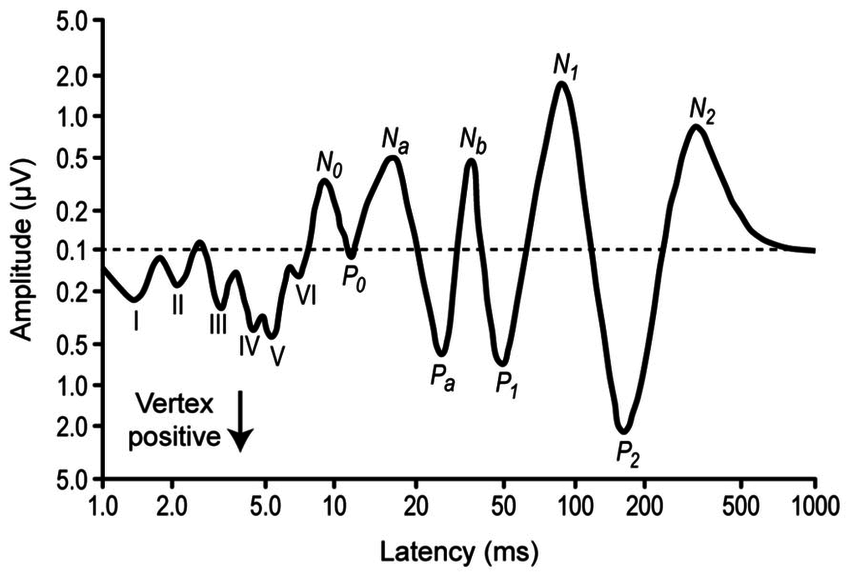
\includegraphics[width=0.8\linewidth]{figuras/AEP.png}
    \caption{Representación del potencial evocado auditivo. Como tal, este gráfico es ideal y no se observa con esta calidad en estudios clínicos. Obtenido de \cite{perez-gonzales-2014}.}
    \label{fig:AEP}
\end{figure}

Las mediciones principales que se realizan sobre el ABR son las latencias, amplitudes y duración de intervalos de las ondas I a III, III a V, y I a V. La latencia se define como el tiempo transcurrido entre que se aplica el estímulo y el pico de una onda. Tanto latencias como amplitudes son afectadas por la edad (mayor edad es igual a mayor latencia y menor amplitud) y la intensidad del estímulo (mayor intensidad es igual a menor latencia y mayor amplitud) \cite{young-ABR}.

Más allá de la tipificación del ABR, la presencia de estos marca que el estímulo sonoro efectivamente causó una respuesta neurofisiológica. Se define como umbral auditivo como la intensidad mínima a partir de la cual un ABR reproducible puede formarse y detectarse \cite{sininger-1993-ABR}.

No obstante, la percepción sonora puede verse afectada por patologías con incidencia en estructuras superiores, tales como el tálamo o la corteza. Esto no quita valor a la evaluación audiométrica a través de ABR. Al contrario, permite discernir con mayor granularidad cuáles son las patologías potenciales que pueden estar afectando al paciente, ya que evalúan el procesamiento sonoro en un punto intermedio entre su recepción y percepción consciente. 

\subsection{Adquisición de la señal fisiológica}

Para obtener una señal de potencial evocado auditivo del tipo ABR, se deben
colocar tres electrodos en el paciente de la siguiente manera:

\begin{itemize}
    \item Electrodo de activo ($V_{in}^{+}$): en la frente del paciente.
    \item Electrodo de tierra ($V_{in}^{-}$): en la apófisis mastoides ipsilateral del paciente.
    \item Electrodo de referencia (neutro): en la apófisis mastoides contralateral del paciente.
\end{itemize}

La señal de ABR se obtiene midiendo la diferencia de potencial entre los electrodos $V_{in}^{+}$ y $V_{in}^{-}$, utilizando como referencia de acoplamiento eléctrico al electrodo neutro. Esta señal es particularmente ruidosa, y su amplitud es del orden de los 500 [nV]. Por ello, se la debe filtrar y amplificar analógicamente previo a su tratamiento digital \cite{shojaeemend_automated_2018}.

Se suele utilizar un filtro pasabandas de 150 a 3000 [Hz] para eliminar ruido de baja y alta frecuencia. Para amplificar, como se explica más adelante, se utiliza una combinación de circuitos integrados para lograr una ganancia total de entre 10000 y 500000.

\subsection{Preprocesamiento digital de la señal}

Una vez que se cuenta con la señal digital, es necesario preacondicionarla previo a procesarla si se desea obtener un análisis con significancia. La relación fisiológica de señal-ruido (SNR por \textit{Signal-to-Noise Ratio}) para el potencial evocado es de -20 dB, considerando que la amplitud estándar del EEG (electroencefalograma) es de 5 $\mu$V \cite{young-ABR} y la del ABR de 0.5 $\mu$V  \cite{bhattacharyya-ABR}. Debido a tal limitación, es importante remover lo más posible el ruido que induce la etapa de adquisición de la señal analógica y su digitalización.

Dado que se necesitan múltiples repeticiones de una misma prueba para obtener un potencial evocado, todo el procesamiento de la señal se realiza de forma \textit{offline}, es decir, con las señales almacenadas por completo en memoria.

Como primera etapa, se introduce usualmente un filtro digital de tipo IIR (de \textit{Infinite Impulse Response}) que se aplica en ambos sentidos para eliminar la pobre respuesta en fase que poseen este tipo de diseños. No obstante, requieren de un menor orden para lograr las mismas especificaciones en amplitud que filtros de tipo FIR (de \textit{Finite Imput Response}) \cite{madsen-2017-AverageEP}.

A continuación, se descartan las repeticiones que posean un umbral mayor a una referencia, para evitar artefactos introducidos por ECG (electrocardiografía) y EMG (electromiografía). El umbral suele asignarse entre 25 y 40 $\mu$V.

\subsection{Obtención del potencial evocado}

Finalmente, se procede a realizar promediación por bloques. Este tipo de procesamiento asume que el ruido es independiente de la señal y aleatorio, por lo que puede removerse si múltiples repeticiones se apilan unas sobre otras \cite{davila-1992-Weigthed-Average}. Existen diversos modelos para elegir los pesos que se aplican a cada iteración, que tienen en cuenta factores como la amplitud del ruido (estimado por la varianza de cada ensayo) y la señal (estimada como el producto punto entre el promedio y cada iteración) \cite{pander-2014-Weigthed-Average}. Para realizar pruebas clínicas, no obstante, se prefiere utilizar un promedio homogéneo, dado que otras técnicas de estimación pueden producir artefactos si la calidad de la señal no es óptima, dando lugar a falsos resultados \cite{norrix-2019-Weigthed-Average}. Luego, el potencial evocado se determina con el promedio homogéneo de todas las repeticiones filtradas y que hayan pasado el umbral de referencia:

\begin{equation}
\hat{s} = \frac{1}{N} \sum_{i=1}^Nx_i
\label{eq:signal_homogeneous_averaging}
\end{equation}

Donde $\hat{s}$ es la señal estimada y $x_i$ son las pruebas preprocesadas.

\subsection{Generación del estímulo auditivo}

Las frecuencias sonoras que suelen evaluarse en una audiometría estándar son 250, 500, 1000, 2000, 4000 y 8000 (aunque a veces se puede extender a 125 y 16000) [Hz] \cite{Cognifit}. 

Es conocido que distintos dispositivos poseen características diferentes en cuanto a la respuesta en frecuencia y potencia de sus salidas de audio. Es por ello que se realiza el desarrollo y testeo de audiómetros manteniendo la misma configuración en cuanto a la generación de audio. 

Por otro lado, la respuesta del oído humano a ondas sonoras de distintas frecuencias es variable, mostrando una percepción desigual ante la misma amplitud \cite{Fechner}. En particular, frecuencias medias y medias altas (2000 a 8000 Hz) tienden a escucharse con mayor intensidad para una misma amplitud en la señal analógica que produce el sonido. Un modelo sencillo que permite ajustar estas diferencias es el de Steven's \cite{Fechner}:

\begin{equation}
N_{dB_0}^f = N_{dB_0}^{f_0} \left(\frac{f}{f_0}\right) ^ \alpha
\label{eq:equivalent_sound_intensity}
\end{equation}

Donde $N_{dB_0}^f$ es el nivel de amplitud de referencia para una determinada frecuencia, $f_0$ es una frecuencia de referencia (usualmente la más baja con la que se trabaja) y $\alpha$ es una constante que varía entre -1 y -2 para el rango de frecuencias evaluado.

Para audiometría clínica profesional, se emplea una técnica de calibración más exhaustiva, en la que se determina el nivel de amplitud de referencia (umbrales de audición normalizados) para cada frecuencia en base al resultado promedio para una muestra (usualmente de diez) con sujetos cuya audición se considera fisiológica (Norma ISO 389 \cite{ISO389}). No obstante, en el presente trabajo no se implementa dicha calibración debido a que excede el alcance del trabajo. En su lugar, te tomó como referencia el promedio entre los límites perceptibles de los desarrolladores, todos normoacúsicos.

En cuanto a la realización de cada prueba, los estímulos deben ser cortos (alrededor de 10 ms), debido a que de lo contrario los ABRs producidos en el tiempo se integran temporalmente dentro del encéfalo y dejan de ser observables. Luego de aplicar cada estímulo debe de introducirse por consiguiente un tiempo de silencio, que suele permanecer entre 15 y 20 ms. Por lo tanto, resulta de gran relevancia que todo el ensayo audiométrico se realice en un ambiente insonoro, ya que de lo contrario no se podrá obtener la respuesta fisiológica del paciente \cite{funasaka-1986}.
\section{Materiales y métodos} \label{materiales_metodos}


\section{Resultados} \label{resultados}
\section{Discusion} \label{discusion}

\section{Conclusion} \label{conclusion}

En base a los resultados obtenidos, se puede concluir que la CABRA es capaz de registrar los ABR con una consistencia aceptable. Además, su costo de fabricación, inferior a 100 USD, representa una diferencia significativa en comparación con los audiómetros comerciales actuales, cuyo precio ronda los 3.000 USD. Dados los resultados obtenidos, es plausible afirmar que se han cumplido los objetivos de mínima planteados. Esto demuestra el potencial de la CABRA. como una alternativa accesible para aplicaciones en regiones de bajos recursos, como Asia, África y América Latina \cite{business-research-insights-audiometers}.

Las tendencias actuales del mercado incluyen la integración de inteligencia artificial (IA) y algoritmos de \textit{Machine Learning}, el diseño de audiómetros más amigables para el uso pediátrico y el aumento de la demanda de dispositivos móviles y portátiles \cite{business-research-insights-audiometers}. Nuestro proyecto responde a estas necesidades al mantener un volumen de 0.8 litros y al incorporar un sistema experto que asiste al usuario en la identificación de los picos en los ABR. No obstante, resta mejorar el sistema para esquematizar cómo podría realizarse una prueba audiométrica completa de forma automática, así como independizar físicamente el dispositivo del ordenador en el que se comandan y visualizan las pruebas. Dichas propuestas constituyen una gran oportunidad para profundizar en el desarrollo del audiómetro y marcan un puntapié por el que se plantea alcanzar un equipo comercial.
\newpage
\section*{Referencias}
\bibliographystyle{IEEEtran}
\nocite{*}
\bibliography{references}

\end{document}